\documentclass{article}
\usepackage{hyperref}
\usepackage{tikz}
\usepackage{amsmath}
\usepackage[a4paper]{geometry}
\usepackage{fancyhdr}
\pagestyle{fancy}
\lhead{Ebenen}
\rhead{April 2025}
\begin{document}
 
\newcommand{\vect}[1]{\overrightarrow{#1}} 
\newcommand{\vectp}[1]{\vect{\mathrm{#1}}}
 
\noindent \begin{minipage}[t]{\dimexpr\textwidth-6cm}
 \vspace{0pt}  
 \section{Ebenen}
 Wird zu einer Parametergleichung einer Gerade ein vielfaches des Vektores $\vectp{AC}$, welcher in eine andere Richtung zeigt, also nicht kollinear ist, hinzugefügt, geht von jedem Punkt der ursprünglichen Gerade je eine weitere, in die Richtung von $\vectp{AC}$ gerichtete zeigend, Gerade aus.
 Diese neue Parametergleichung kann somit alle Punkte, welche einer auf einer unendlichen zwei dimensionalen Ebene liegen, darstellen. \newline
 Sie folgt oftmals der Parameterform  
 \[
  E: \vect{x} = \vectp{OA} + r \cdot \vectp{AB} + s \cdot \vectp{AC} 
 \]
\end{minipage}
\hfill
\begin{minipage}[t]{6cm}
  \centering
  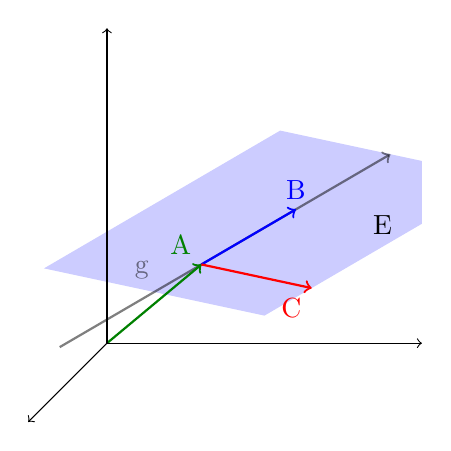
\begin{tikzpicture}[baseline=(current bounding box.north)]
 
    \begin{scope} 
      \clip(-1,0) rectangle (4,4);
      \fill[blue!20] (1.2-0.5*1.2-1.4,1-0.5*0.7+0.3) -- (1.2+2*1.2-1.4,1+2*0.7+0.3) -- (1.2+2*1.2+1.4,1+2*0.7-0.3) -- (1.2-0.5*1.2+1.4,1-0.5*0.7-0.3) -- cycle;
      \draw (3.5, 1.5) node[black, opacity=1,] {E}; 
    \end{scope} 
 
    \draw[->,thick,black,opacity=0.5] (1.2-1.2*1.5,1-0.7*1.5) -- (1.2+1.2*2,1+0.7*2) node[pos=0.3, above left] {g};
    \draw[->,thick,green!50!black] (0,0) -- (1.2,1) node[above left] {$\mathrm{A}$};
    \draw[->,thick,blue] (1.2,1) -- ++(1.2,0.7) node[above] {$\mathrm{B}$};
    \draw[->,thick,red] (1.2,1) -- ++(1.4,-0.3) node[below left] {$\mathrm{C}$};
 
    \draw[->] (0,0) -- (4,0);
    \draw[->] (0,0) -- (0,4);
    \draw[->] (0,0) -- (-1, -1);
  \end{tikzpicture}
\end{minipage}
 
\vspace{1em}  
\noindent Ein Punkt liegt auf der Ebene, wenn es möglich ist diesen mit der Parametergleichung der Ebene gleich zu setzen und jeweils einen Wert für $r$ und $s$ zu finden.
 
\subsection{Parametergleichung}
Um die Parametergleichung einer Ebene zu finden, müssen der Stützvektor und zwei Richtungsvektoren, welche nicht zueinander kollinear sind, bestimmt werden. Sind drei Punkte gegeben, welche nicht auf einer Gerade liegen, kann einer davon, normalerweise $\mathrm{A}$, als Stützvektor genutzt werden, wobei die jeweiligen Verbindungsvektoren zu den zwei anderen Punkten als Richtungsvektoren verwendet werden können, wie oben gezeigt. \newline
Sind hingegen nicht drei Punkte gegeben, sondern ein Punkt und eine Gerade oder garkeine Punkte und zwei Geraden, so können selbst Punkte auf der Gerade bestimmt werden, welche genutzt werden können, um auf einen Stützvektor und zwei Richtungsvektoren zu kommen.
 
\subsection{Normalform}
Offensichtlich ist jeder Verbindungsvektor zwischen zwei Punkten einer Ebene $\mathrm{E}$ zu dem Normalvektor $\vect{n}$ dieser Ebene orthogonal, heißt hat ein Skalarprodukt von null. Somit gilt für jeden Punkt $\vect{x}$ auf der Ebene $\mathrm{E}$ mit einem Stützvektor $\vect{p}$
\[
 (\vect{x} - \vect{p}) \cdot \vect{n} = 0 
\]
In dieser Form ist auch zugleich der Normalvektor $\vect{n}$ sehr einfach abzulesen. 
 
\subsection{Koordinatenform}
Eine Ebenengleichung kann auch als
\[
 n_1 \, x_1 + n_2 \, x_2 + n_3 \, x_3 = e 
\]
aufgeschrieben werden, wobei mit einem beliebigen Stützvektor $\vect{p}$ der Ebene $e = \vect{p} \cdot \vect{n}$ gilt. Manchmal wird $n_1 \, x_1 + n_2 \, x_2 + n_3 \, x_3$ auch zu $\vect{x} \cdot \vect{n}$ gekürzt. Wird die Koordinatenform aus $\vect{x} \cdot \vect{n} = \vect{p} \cdot \vect{n}$ wird es offensichtlich dass sie in wenigen Schritten aus der Normalform gebildet werden kann.
 
\subsection{Hesse'sche Normalform}
Hierzu mehr im Kapitel \hyperref[Abstände zwischen Punkten und Ebenen]{Abstände zwischen Punkten und Ebenen}. Die Hesse'sche Normalform besagt dass mit einem Punkt $\mathrm{P}$ als Stützvektor der Ebene
\[
 \frac{1}{|\vect{n}|} (\vect{n} \cdot \vect{x} - \vect{n} \cdot \vectp{OP}) = 0 
\]
Hier ist zu beachten, dass dies eigentlich nur die Normalform, umgeformt und multipliziert mit $\dfrac{1}{|\vect{n}|}$ ist.
 
\subsection{Umformung}
Weil sowohl die Normalform, die Koordinatenform und die Hesse'sche Normalform sich direkt oder indirekt  auf $\vect{x}$, $\vect{n}$ und $\vect{p}$ beziehen, können diese immer identifiziert und in die Formel der jeweils anderen Form eingesetzt werden. 
 
Im Falle der Koordinatengleichung kann ein $\vect{p}$ bestimmt werden, indem nach einem $\vect{x}$ gesucht wird, für welches die Gleichung eine Identität darstellt, am einfachsten indem zwei der Koordinaten zu null gesetzt werden und die eine überbleibende aufgelöst wird.
 
Die Richtungsvektoren der Parameterform können mithilfe von $\vect{n}$ gefunden werden; sie sind immer zwei zu $\vect{n}$ orthogonale, aber nicht zueinander kollineare, Vektoren. In anbetracht der Funktionsweise eines Skalarproduktes, kann offensichtlich ein orthogonaler Vektor gefunden werden, indem eine Koordinate gleich null gesetzt wird und die anderen beiden vertauscht werden, wobei eine der beiden negativ gesetzt wird.
 
Somit können die Richtungsvektoren einer Ebene mit dem Normalvektor $\vect{n}$ 
\[
 \begin{pmatrix} 0 \\ -n_3 \\ n_2 \end{pmatrix}
 \quad \text{und} \quad
 \begin{pmatrix} -n_3 \\ 0 \\ n_1 \end{pmatrix} 
 \quad \text{und} \quad
 \begin{pmatrix} n_2 \\ -n_1 \\ 0 \end{pmatrix}  
\]
und alle dazugehörigen Gegenvektoren sein, weil, per definition,
\begin{align*} 
 \begin{pmatrix} n_1 \\ n_2 \\ n_3 \end{pmatrix}
 \cdot
 \begin{pmatrix} -n_3 \\ 0 \\ n_1 \end{pmatrix}
 &= (n_1 \cdot -n_3) + (n_2 \cdot 0) + (n_3 \cdot n_1) \\
 &= -(n_1 \cdot n_3) + 0 + (n_3 \cdot n_1) \\
 &= (n_1 \cdot n_3) - (n_1 \cdot n_3) \\
 &= 0 
\end{align*}  
\end{document} 
 
 
